\chapter{Геодезические, равномерное ускорение и ньютоновский предел}

Непосредственная проблема — гравитация. Точнее, нам нужна метрика пространства-времени, описывающая почти однородное гравитационное поле, например поле в небольшой лаборатории вблизи поверхности Земли. Как оказывается, кратчайший путь к этой метрике не является прямым. Сначала мы должны придать операциональный смысл трём геометрическим идеям: ковариантному дифференцированию, параллельному переносу и геодезическому движению.

Эти идеи зависят друг от друга. Ковариантное дифференцирование говорит нам, как сравнивать векторы в соседних точках. Параллельный перенос говорит, как переносить вектор, не поворачивая его. Геодезическая получается тогда, когда переносимый вектор является касательным к самой траектории. Как только траектория лежит в пространстве-времени, а не в пространстве, то же самое уравнение геодезической становится уравнением движения свободно падающей частицы.

Во второй половине лекции затем делается поразительный шаг. Мы остаёмся в плоском пространстве-времени Минковского, но описываем его координатами, приспособленными к жёстко ускоренному семейству наблюдателей. В этих координатах метрика выглядит гравитационной. Вблизи одного из наблюдателей она воспроизводит потенциал однородного поля, а её геодезические удовлетворяют ньютоновскому уравнению
\begin{equation}
\frac{d^2y}{d\tau^2}=-g.
\end{equation}
Это принцип эквивалентности, записанный в виде вычисления.

\section{Ковариантная производная: напоминание}

В выбранной точке \(P\) можно выбрать координаты, максимально близкие к декартовым. В лекции сначала используется выражение «гауссовы нормальные координаты», а затем сразу же делается оговорка. Название менее важно, чем локальные условия:
\begin{equation}
g_{mn}(P)=\delta_{mn},
\qquad
\partial_r g_{mn}(P)=0.
\label{eq:l4-normal-point}
\end{equation}
Это нормальные координаты в одной точке. Они не обязаны оставаться декартовыми в конечной окрестности, и таких реперов существует много, поскольку их оси можно поворачивать.

Метрика совместима с оператором производной:
\begin{equation}
\nabla_r g_{mn}=0,
\qquad
\nabla_r g^{mn}=0.
\label{eq:l4-metric-compatibility}
\end{equation}
Для ковектора \(V_s\) ковариантная производная имеет вид
\begin{equation}
\nabla_r V_s
=
\partial_r V_s-\Gamma^p{}_{rs}V_p.
\label{eq:l4-covector-derivative}
\end{equation}
Коэффициенты связности равны
\begin{equation}
\Gamma^p{}_{rs}
=
\frac{1}{2}g^{pn}
\left(
\partial_s g_{nr}
+\partial_r g_{ns}
-\partial_n g_{rs}
\right).
\label{eq:l4-christoffel}
\end{equation}
При записи этого выражения на доске исправляются несколько индексов. Уравнение \eqref{eq:l4-christoffel} даёт окончательное соотношение. Оно симметрично по \(r\) и \(s\), как и следует ожидать для связности Леви-Чивиты без кручения.

\begin{figure}[htbp]
\centering
\includegraphics[width=0.92\textwidth]{lecture_04_figure_01.png}
\caption{Ковариантная производная ковектора и окончательная формула для символов Кристоффеля.}
\end{figure}

Поскольку символы Кристоффеля строятся из первых производных метрики, они обращаются в нуль в \(P\) в координатах \eqref{eq:l4-normal-point}. Они не обращаются в нуль в любой системе координат, даже когда лежащее в основе пространство плоское. Следовательно, \(\Gamma^p{}_{rs}\) не является тензором. Именно этот нетензорный характер позднее и позволит ускоренному наблюдателю описывать гравитационную силу, которую инерциальный наблюдатель не видит.

\subsection{Поднятие векторного индекса}

Соответствующая производная вектора вводится не как отдельное правило, которое нужно заучивать. Она следует из метрики. Начнём с
\begin{equation}
V^n=g^{np}V_p.
\end{equation}
Тогда
\begin{align}
\nabla_m V^n
&=\nabla_m\!\left(g^{np}V_p\right) \\
&=(\nabla_m g^{np})V_p+g^{np}\nabla_m V_p \\
&=g^{np}\left(\partial_mV_p-\Gamma^r{}_{mp}V_r\right),
\end{align}
где метрическая совместимость устранила первый член. Перегруппировав индексы, получаем
\begin{equation}
\nabla_m V^n
=
\partial_m V^n+\Gamma^n{}_{mr}V^r.
\label{eq:l4-vector-derivative}
\end{equation}

\begin{figure}[htbp]
\centering
\includegraphics[width=0.90\textwidth]{lecture_04_figure_02.png}
\caption{Поднятие индекса с помощью обратной метрики перед дифференцированием.}
\end{figure}

\begin{figure}[htbp]
\centering
\includegraphics[width=0.90\textwidth]{lecture_04_figure_03.png}
\caption{Ковариантная производная для верхнего индекса, вытекающая из метрической совместимости и правила произведения.}
\end{figure}

Итак, правило для индексов просто:
\begin{equation}
\boxed{
\begin{aligned}
\text{lower index:}&\quad -\Gamma,\\
\text{upper index:}&\quad +\Gamma.
\end{aligned}}
\end{equation}
Для тензора более высокого ранга по одному члену со связностью появляется для каждого индекса, а его знак определяется тем, является ли этот индекс нижним или верхним.

\subsection{Вопрос терминологии}

Что именно представляют собой упомянутые выше наилучшие координаты? Здесь не утверждается, что они образуют некоторую выделенную глобальную систему координат. В одной выбранной точке они делают метрику равной её плоской форме и обращают в нуль её первые производные. Поворот осей даёт другой столь же хороший репер. Геометрические утверждения, полученные в таком репере, не зависят от этой ориентации, потому что конечные объекты являются тензорами.

\section{Параллельный перенос вдоль кривой}

Пусть вектор \(V^n\) переносится вдоль кривой. При бесконечно малом смещении \(dx^m\) его ковариантное изменение равно
\begin{align}
\delta V^n
&=(\nabla_mV^n)\,dx^m \\
&=\partial_mV^n\,dx^m
+\Gamma^n{}_{mr}V^r\,dx^m \\
&=dV^n+\Gamma^n{}_{mr}V^r\,dx^m.
\label{eq:l4-covariant-differential}
\end{align}

\begin{figure}[htbp]
\centering
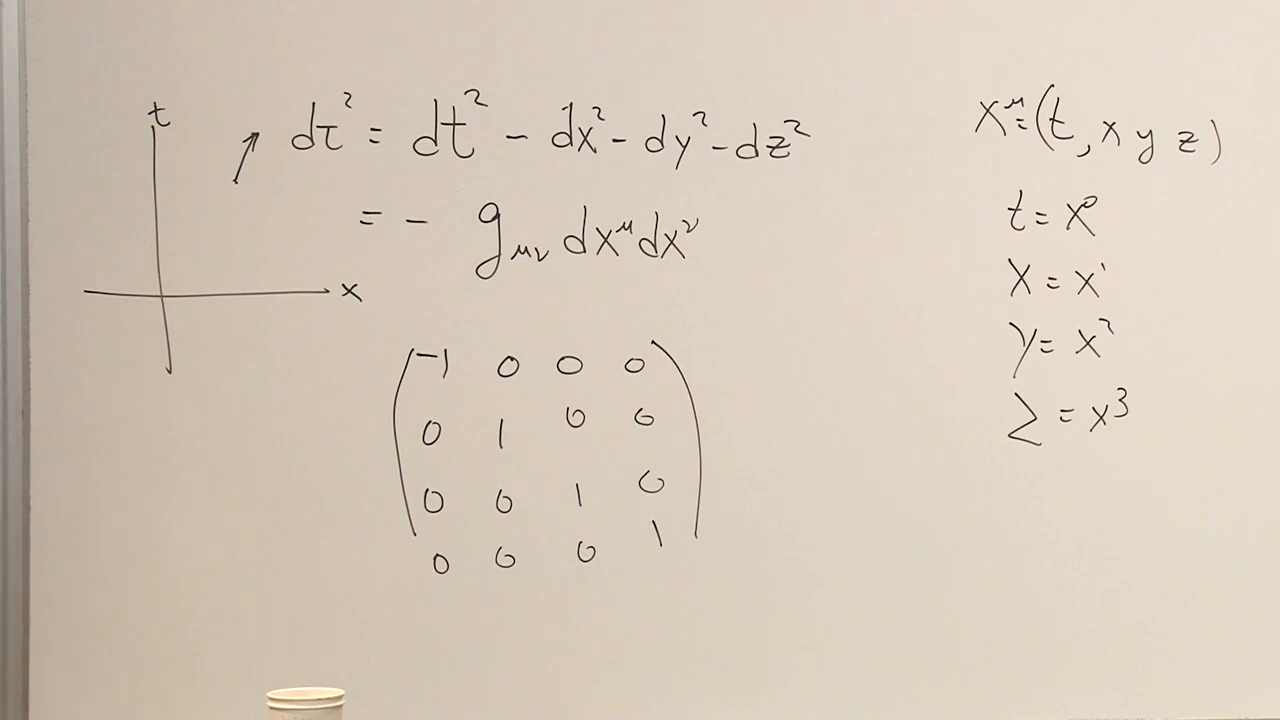
\includegraphics[width=0.92\textwidth]{lecture_04_figure_04.png}
\caption{Обычное изменение компонент и поправка связности вдоль кривой.}
\end{figure}

Вектор переносится параллельно, когда это ковариантное изменение равно нулю:
\begin{equation}
\boxed{
dV^n+\Gamma^n{}_{mr}V^r\,dx^m=0.
}
\label{eq:l4-parallel-transport}
\end{equation}
Операционально можно вообразить, что в каждой точке кривой мы строим нормальный репер. В этом локальном репере требуется, чтобы переносимый вектор не поворачивался. Затем мы смещаемся на бесконечно малое расстояние, строим следующий нормальный репер и повторяем.

\begin{figure}[htbp]
\centering
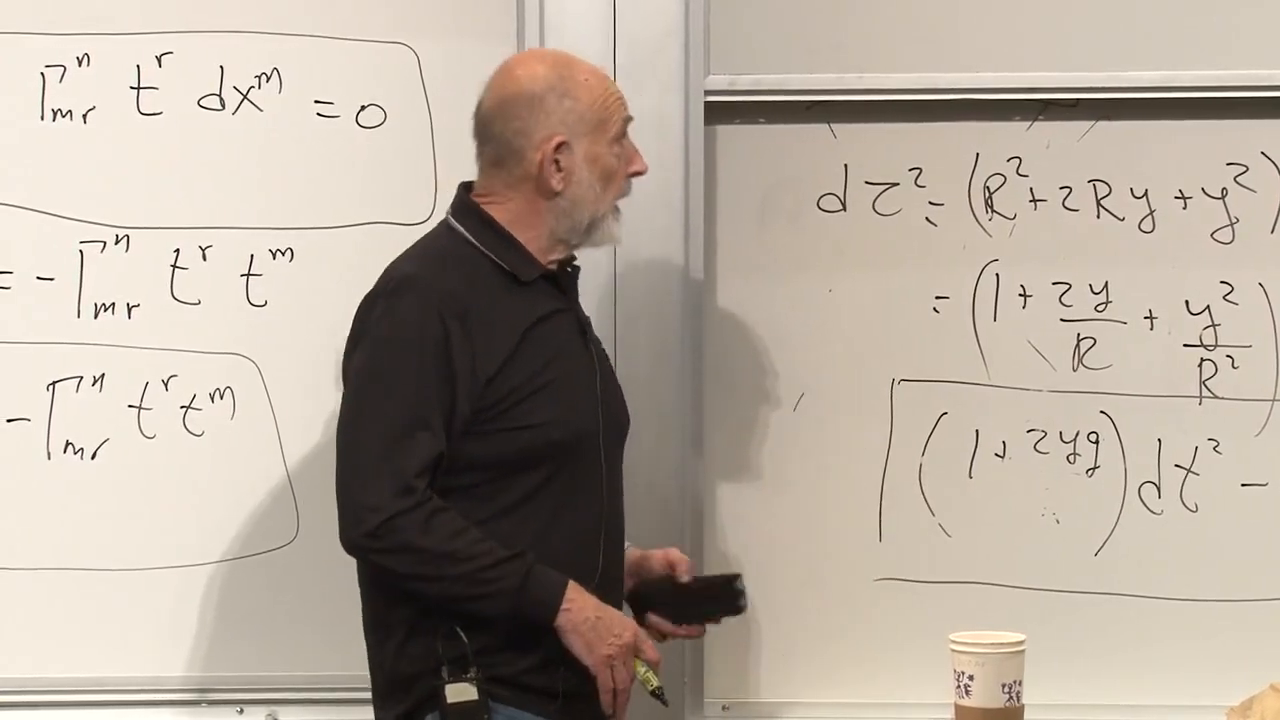
\includegraphics[width=0.92\textwidth]{lecture_04_figure_05.png}
\caption{Чёткая запись на доске уравнения параллельного переноса.}
\end{figure}

Ориентация каждого временного нормального репера не относится к физике. Перед сравнением мы могли бы повернуть его. Существенно то, что ковариантное утверждение \eqref{eq:l4-parallel-transport} не зависит от этого произвольного выбора.

\subsection{Зависимость от пути и кривизна}

В искривлённом пространстве параллельный перенос зависит от пути. Возьмём один и тот же вектор в одной и той же начальной точке и перенесём его в ту же конечную точку по двум различным маршрутам. Вообще говоря, конечные векторы различаются. При переносе вектора по замкнутому контуру он может вернуться повернутым. Это несовпадение — голономия, и оно является прямым признаком кривизны.

\begin{figure}[htbp]
\centering
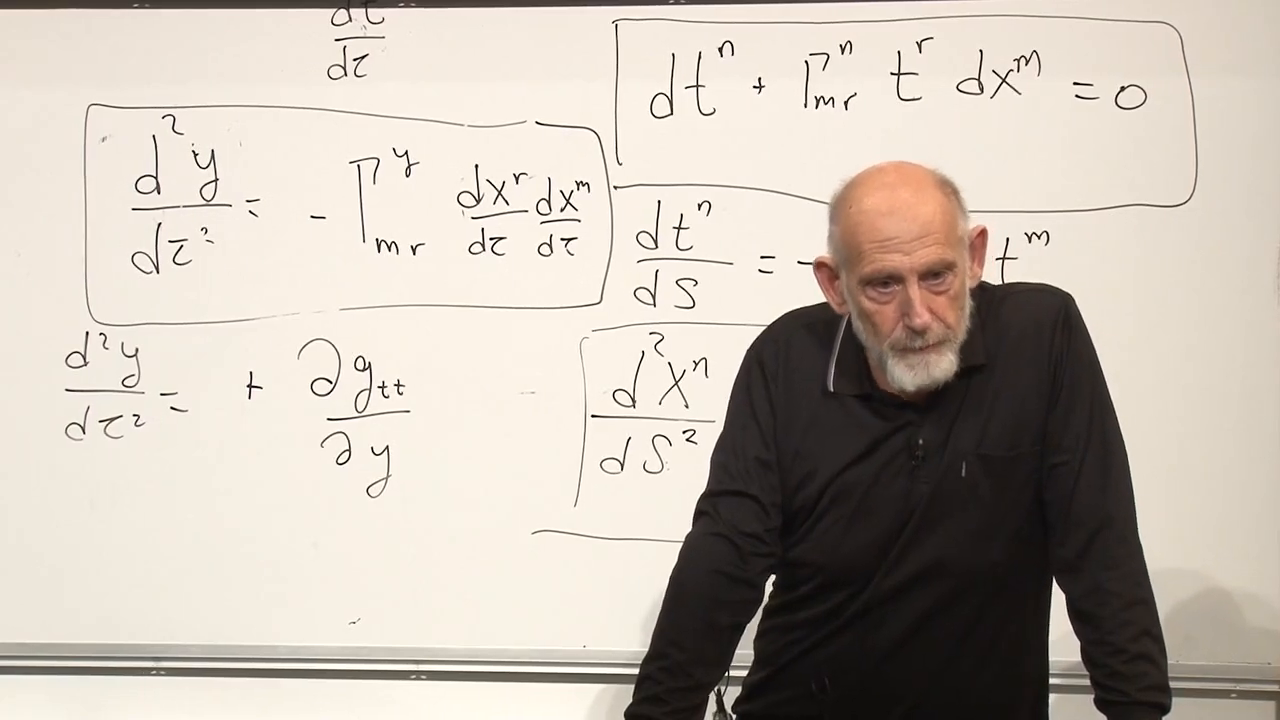
\includegraphics[width=0.90\textwidth]{lecture_04_figure_06.png}
\caption{Два маршрута на искривлённой поверхности не обязаны переносить вектор к одной и той же конечной ориентации.}
\end{figure}

Конус даёт полезный пример. Вдали от вершины конус можно разрезать и развернуть на плоскость. Тем не менее параллельный перенос по петле, охватывающей вершину, возвращает вектор, повернутый на величину углового дефицита. Если вершина сглажена, кривизна конечна и распределена по малой области. Если она идеально острая, идеализация сосредоточивает кривизну в вершине.

\begin{figure}[htbp]
\centering
\includegraphics[width=0.90\textwidth]{lecture_04_figure_07.png}
\caption{Круговое движение на конусе и его развёртка на плоскости после разрезания.}
\end{figure}

\subsection{Вопросы о переносимом векторе}

\paragraph{Должен ли вектор быть определён всюду?}
Нет. Можно начать с одного вектора в одной точке и решать \eqref{eq:l4-parallel-transport} только вдоль выбранной кривой. Полное векторное поле не обязательно. Если поле определено в некоторой области, оно может быть ковариантно постоянным в одном направлении и не быть таковым в другом.

\paragraph{Сохраняется ли его длина?}
Да. Пусть \(V^2=g_{mn}V^mV^n\). Вдоль кривой,
\begin{align}
\frac{D}{d\lambda}\left(g_{mn}V^mV^n\right)
&=
\frac{Dg_{mn}}{d\lambda}V^mV^n
+2g_{mn}V^m\frac{DV^n}{d\lambda}\\
&=0.
\end{align}
Метрическая совместимость обращает в нуль первый член, а параллельный перенос — второй. Следовательно, длины и взаимные углы параллельно переносимых векторов сохраняются.

\paragraph{Параллельно ли переносится касательный вектор к любой кривой?}
Нет. Этот вопрос прямо приводит к геодезическим. Касательный вектор к круговому пути вокруг конуса непрерывно поворачивается. Касательный вектор к прямой линии, получающейся после разрезания конуса, не поворачивается. Только второй путь является локально прямым.

\section{Геодезические: прямейшие, а не просто кратчайшие}

У геодезической есть два связанных описания. Глобально это стационарная кривая функционала длины или собственного времени. Локально это максимально прямая из возможных траекторий. Слово «стационарная» важно: в зависимости от геометрии и конечных точек траектория не обязана быть единственным глобальным минимумом. В лоренцевом пространстве-времени времениподобные геодезические локально максимизируют собственное время, а не минимизируют положительную длину.

Здесь нужно именно локальное описание. Небольшой автомобиль, движущийся по искривлённой местности с рулём, удерживаемым строго прямо, идёт по геодезической, при условии что размеры автомобиля малы по сравнению с масштабом, на котором изгибается местность. В пространстве вложения такая линия не обязана выглядеть прямой; она прямая в смысле геометрии самой поверхности.

\begin{figure}[htbp]
\centering
\includegraphics[width=0.90\textwidth]{lecture_04_figure_08.png}
\caption{Путь на искривлённой поверхности, заданный внутренней геометрией, подготавливает определение прямейшего пути.}
\end{figure}

\subsection{Касательный вектор}

Пусть кривая задаётся как \(x^m(s)\), а элемент длины дуги равен
\begin{equation}
ds^2=g_{mn}\,dx^m dx^n.
\end{equation}
Единичный касательный вектор имеет вид
\begin{equation}
t^m=\frac{dx^m}{ds}.
\label{eq:l4-unit-tangent}
\end{equation}
Геометрически: возьмём две близкие точки, составим вектор смещения между ними, разделим его на расстояние между ними и устремим точки друг к другу.

\begin{figure}[htbp]
\centering
\includegraphics[width=0.90\textwidth]{lecture_04_figure_09.png}
\caption{Касательное направление как предельное смещение вдоль кривой.}
\end{figure}

\begin{figure}[htbp]
\centering
\includegraphics[width=0.90\textwidth]{lecture_04_figure_10.png}
\caption{Линейный элемент и единичный касательный вектор \(t^m=dx^m/ds\).}
\end{figure}

Геодезическая — это кривая, касательный вектор которой параллельно переносится вдоль неё самой:
\begin{equation}
dt^n+\Gamma^n{}_{mr}t^r\,dx^m=0.
\end{equation}
Разделим на \(ds\) и используем \(dx^m/ds=t^m\):
\begin{equation}
\frac{dt^n}{ds}
=
-\Gamma^n{}_{mr}t^m t^r.
\end{equation}
Наконец, подставим \(t^n=dx^n/ds\):
\begin{equation}
\boxed{
\frac{d^2x^n}{ds^2}
+\Gamma^n{}_{mr}
\frac{dx^m}{ds}
\frac{dx^r}{ds}
=0.
}
\label{eq:l4-geodesic}
\end{equation}

\begin{figure}[htbp]
\centering
\includegraphics[width=0.94\textwidth]{lecture_04_figure_11.png}
\caption{Закон переноса касательного вектора и геодезическое уравнение второго порядка.}
\end{figure}

Уравнение \eqref{eq:l4-geodesic} уже напоминает ньютоновскую динамику. Если вместо \(s\) взять подходящий временной параметр, первый член будет ускорением. Член со связностью тогда действует как сила на единицу массы, полностью определяемая метрикой. В общей теории относительности эта аналогия становится буквальной: свободные частицы следуют геодезическим пространства-времени, а то, что Ньютон называл гравитационным ускорением, проявляется через связность.

\section{От риманова расстояния к собственному времени пространства-времени}

Теперь обсуждение переходит от искривлённого пространства к пространству-времени. В инерциальных декартовых координатах собственное время между близкими событиями равно
\begin{equation}
d\tau^2
=dt^2-dx^2-dy^2-dz^2.
\label{eq:l4-proper-time}
\end{equation}
В лекции используется
\begin{equation}
d\tau^2=-g_{\mu\nu}\,dx^\mu dx^\nu
\label{eq:l4-lecture-sign}
\end{equation}
при
\begin{equation}
g_{\mu\nu}
=
\eta_{\mu\nu}
=
\begin{pmatrix}
-1&0&0&0\\
0&1&0&0\\
0&0&1&0\\
0&0&0&1
\end{pmatrix}.
\label{eq:l4-eta}
\end{equation}
Таким образом, внешний знак минус в \eqref{eq:l4-lecture-sign} превращает выбранную метрику с преобладанием плюсов в \eqref{eq:l4-proper-time}. Координаты таковы:
\begin{equation}
\begin{aligned}
x^\mu&=(t,x,y,z),\\
x^0&=t,\quad x^1=x,\\
x^2&=y,\quad x^3=z.
\end{aligned}
\end{equation}

\begin{figure}[htbp]
\centering
\includegraphics[width=0.94\textwidth]{lecture_04_figure_12.png}
\caption{Собственное время, координаты пространства-времени и метрика Минковского с преобладанием плюсов.}
\end{figure}

Сигнатура — это инвариантная информация: одно собственное значение имеет знак, связанный со временем, а три — знак, связанный с пространством. Умножив всю метрику на \(-1\) и согласованно изменив все соглашения, получаем столь же распространённую конвенцию с преобладанием минусов. Ничто физическое от этого общего выбора не зависит.

На лекции задаётся вопрос, рассматривались ли пространства с другими неопределёнными сигнатурами. Математически псевдоримановы геометрии со многими сигнатурами хорошо изучены. В физическом отношении вопрос уже: наблюдаемое релятивистское пространство-время лоренцево и имеет одно временное направление. Дополнительные времениподобные направления глубоко изменили бы причинную структуру и не описывают обсуждаемую здесь физику.

\begin{figure}[htbp]
\centering
\includegraphics[width=0.94\textwidth]{lecture_04_figure_13.png}
\caption{Соглашение о знаках проверяется перед тем, как плоская метрика обозначается через \(\eta_{\mu\nu}\).}
\end{figure}

Плоское пространство-время не означает, что компоненты метрики обязаны иметь вид \(\eta_{\mu\nu}\) в любой системе координат. Это означает, что существуют такие координаты, в которых они имеют такой вид. Криволинейные или ускоренные координаты могут сделать компоненты зависящими от положения даже тогда, когда тензор Римана равен нулю.

\section{Почему одинаковое координатное ускорение не даёт жёсткого движения}

Мы хотим ввести координаты, связанные с ускоряющимся лифтом. Первая идея — выстроить ряд наблюдателей на фиксированных расстояниях друг от друга и задать им всем одно и то же координатное ускорение. Теория относительности не позволяет этой наивной конструкции оставаться жёсткой.

\begin{figure}[htbp]
\centering
\includegraphics[width=0.92\textwidth]{lecture_04_figure_14.png}
\caption{Ряд соседних наблюдателей, используемый для проверки того, сохраняет ли общее ускорение жёсткость.}
\end{figure}

Если разнесённые наблюдатели, согласно одной инерциальной системе отсчёта, следуют одинаковым программам ускорения, расстояние между ними в их изменяющихся мгновенных системах покоя не остаётся постоянным. Нить, соединяющая их, растягивается и в конце концов рвётся. Это то же кинематическое напряжение, которое проявляется в мысленном эксперименте Белла с космическими кораблями. Более того, постоянное ньютоновское координатное ускорение не может продолжаться сколь угодно долго: в конце концов оно предсказало бы скорость, большую скорости света.

Следовательно, релятивистски жёсткая ускоренная система отсчёта должна иметь в каждой точке разное собственное ускорение. Наблюдатели, находящиеся ближе к предполагаемому горизонту, ускоряются сильнее; те, что дальше, — слабее. Тогда их собственные расстояния могут оставаться постоянными в мгновенно сопутствующей системе отсчёта. Это ускорение, жёсткое в смысле Борна, в одном пространственном измерении.

\section{Евклидовы полярные координаты как подготовительный пример}

Правильную конструкцию легче всего увидеть, начав с обычной окружности. На евклидовой плоскости
\begin{equation}
x=r\cos\theta,
\qquad
y=r\sin\theta,
\end{equation}
поэтому
\begin{equation}
x^2+y^2=r^2,
\qquad
\cos^2\theta+\sin^2\theta=1.
\end{equation}
Комплексно-экспоненциальные представления имеют вид
\begin{equation}
\cos\theta=\frac{e^{i\theta}+e^{-i\theta}}{2},
\qquad
\sin\theta=\frac{e^{i\theta}-e^{-i\theta}}{2i}.
\label{eq:l4-euler-trig}
\end{equation}
Множитель \(i\) в знаменателе формулы для синуса замечается и восстанавливается в ходе обсуждения у доски.

\begin{figure}[htbp]
\centering
\includegraphics[width=0.94\textwidth]{lecture_04_figure_15.png}
\caption{Окружность, евклидовы полярные координаты и их экспоненциальные тригонометрические формы.}
\end{figure}

Фиксированное значение \(r\) задаёт окружность. Движение с постоянной угловой скоростью имеет центростремительное ускорение постоянной величины, всегда направленное внутрь. В пространстве-времени соответствующую роль будет играть гипербола.

\section{Гиперболические координаты в пространстве-времени Минковского}

Заменим тригонометрические функции их гиперболическими аналогами:
\begin{equation}
\cosh\omega=\frac{e^\omega+e^{-\omega}}{2},
\qquad
\sinh\omega=\frac{e^\omega-e^{-\omega}}{2},
\end{equation}
при
\begin{equation}
\cosh^2\omega-\sinh^2\omega=1.
\label{eq:l4-hyperbolic-identity}
\end{equation}
Множителя \(i\) нет. Координата \(\omega\) — это гиперболический угол, или быстрота. В отличие от обычного угла она не периодична; её значения лежат в пределах от \(-\infty\) до \(+\infty\).

\begin{figure}[htbp]
\centering
\includegraphics[width=0.94\textwidth]{lecture_04_figure_16.png}
\caption{Тригонометрические функции в конструкции пространства-времени заменяются гиперболическими.}
\end{figure}

Введём новые координаты в правом клине Риндлера:
\begin{equation}
x=r\cosh\omega,
\qquad
t=r\sinh\omega,
\qquad
r>0.
\label{eq:l4-rindler-transform}
\end{equation}
Тогда
\begin{equation}
x^2-t^2=r^2.
\label{eq:l4-rindler-hyperbola}
\end{equation}
При фиксированном \(r\) изменение \(\omega\) описывает гиперболу. Увеличение \(r\) перемещает поперёк этого семейства в пространственноподобном направлении, тогда как увеличение \(\omega\) продвигает вперёд вдоль одной гиперболы во времениподобном направлении.

\begin{figure}[htbp]
\centering
\includegraphics[width=0.94\textwidth]{lecture_04_figure_17.png}
\caption{Координатное преобразование \(x=r\cosh\omega\), \(t=r\sinh\omega\) и соответствующая ему инвариантная гипербола.}
\end{figure}

\begin{figure}[htbp]
\centering
\includegraphics[width=0.94\textwidth]{lecture_04_figure_18.png}
\caption{Конгруэнция гипербол с фиксированным \(r\), представляющая жёстко ускоренное семейство.}
\end{figure}

\subsection{Метрика в ускоренных координатах}

Продифференцируем \eqref{eq:l4-rindler-transform}:
\begin{align}
dx&=\cosh\omega\,dr+r\sinh\omega\,d\omega,\\
dt&=\sinh\omega\,dr+r\cosh\omega\,d\omega.
\end{align}
Используя \eqref{eq:l4-hyperbolic-identity}, смешанные члены сокращаются:
\begin{align}
d\tau^2
&=dt^2-dx^2\\
&=r^2\,d\omega^2-dr^2.
\label{eq:l4-rindler-metric}
\end{align}
Поперечные направления, если их восстановить, просто добавляют \(-dy^2-dz^2\) к принятому здесь соглашению для собственного времени.

Это по-прежнему плоское пространство-время. Зависящий от координаты коэффициент \(r^2\) свидетельствует о кривизне не больше, чем \(r^2\) перед \(d\theta^2\) в евклидовых полярных координатах.

\subsection{Собственное ускорение вдоль гипербол}

Для фиксированной мировой линии \(r=R\) уравнение \eqref{eq:l4-rindler-metric} даёт
\begin{equation}
d\tau=R\,d\omega.
\end{equation}
Её четырёхскорость равна
\begin{equation}
U^\mu
=
\frac{d(t,x)}{d\tau}
=
(\cosh\omega,\sinh\omega),
\end{equation}
а её четырёхускорение равно
\begin{equation}
A^\mu
=
\frac{dU^\mu}{d\tau}
=
\frac{1}{R}(\sinh\omega,\cosh\omega).
\end{equation}
Инвариантная норма постоянна:
\begin{equation}
a=\sqrt{A^\mu A_\mu}=\frac{1}{R}
\qquad (c=1).
\label{eq:l4-proper-acceleration}
\end{equation}

\begin{figure}[htbp]
\centering
\includegraphics[width=0.90\textwidth]{lecture_04_figure_19.png}
\caption{Закон обратной зависимости от радиуса \(a=1/R\) для фиксированной ускоренной мировой линии.}
\end{figure}

После восстановления единиц
\begin{equation}
\boxed{a=\frac{c^2}{R}.}
\label{eq:l4-proper-acceleration-units}
\end{equation}

\begin{figure}[htbp]
\centering
\includegraphics[width=0.90\textwidth]{lecture_04_figure_20.png}
\caption{При восстановлении единиц \(1/R\) превращается в \(c^2/R\).}
\end{figure}

Чем меньше отсечка \(R\), тем резче изгибается мировая линия и тем больше собственное ускорение, ощущаемое её наблюдателем. Более удалённые гиперболы изгибаются слабее и требуют меньшего ускорения. У каждого наблюдателя ускорение постоянно во времени, но у разных наблюдателей оно различно. Именно это различие и сохраняет их взаимные собственные расстояния.

\subsection{Вопросы об ускоренных координатах}

\paragraph{Является ли \(R\) отсечкой на оси \(x\)?}
Да. При \(\omega=0\) уравнение \eqref{eq:l4-rindler-transform} даёт \(t=0\) и \(x=R\). Эта отсечка определяет собственное ускорение через \eqref{eq:l4-proper-acceleration-units}.

\paragraph{Зависит ли построение от выбранного начала координат?}
Координаты — да. Перенос начала координат порождает другое семейство гипербол со сдвинутыми асимптотами. Никакая инвариантная физика от этого выбора не зависит. Мы намеренно выбираем одну ускоренную систему координат и спрашиваем, как выглядит инерциальное движение при описании в ней.

\paragraph{Что такое собственное ускорение?}
Это ускорение, измеряемое акселерометром, который наблюдатель несёт с собой. В ковариантной форме
\begin{equation}
A^\mu=\frac{dU^\mu}{d\tau},
\qquad
U^\mu=\frac{dx^\mu}{d\tau}.
\end{equation}
Его модуль — это толчок, который наблюдатель действительно ощущает, а не координатное ускорение \(d^2x/dt^2\), приписываемое удалённой системой отсчёта.

\section{Плоские метрики в полярных и гиперболических координатах}

Прежде чем переходить к локализации вблизи Земли, полезно поставить рядом евклидову и лоренцеву метрики. На плоскости,
\begin{equation}
ds^2=dr^2+r^2d\theta^2,
\qquad
g_{ab}
=
\begin{pmatrix}
1&0\\
0&r^2
\end{pmatrix}.
\label{eq:l4-polar-metric}
\end{equation}
Реплика из аудитории ненадолго вводит сферический множитель, но здесь речь идёт только о плоскости, а не о сфере. Член \(r^2\) отражает тот факт, что при большем радиусе фиксированный угловой интервал охватывает более длинную дугу.

\begin{figure}[htbp]
\centering
\includegraphics[width=0.94\textwidth]{lecture_04_figure_21.png}
\caption{Евклидова полярная метрика: компоненты, зависящие от положения, на плоскости.}
\end{figure}

Аналог в пространстве Минковского имеет вид
\begin{equation}
d\tau^2=r^2d\omega^2-dr^2.
\end{equation}
Обе метрики имеют компоненты, зависящие от положения, однако обе геометрии плоские. Координатная кривизна и геометрическая кривизна — не одно и то же.

\section{Локализация вблизи земного ускорения}

Выберем одну опорную гиперболу, собственное ускорение которой равно земному значению \(g\):
\begin{equation}
g=\frac{c^2}{R},
\qquad
R=\frac{c^2}{g}.
\label{eq:l4-earth-radius}
\end{equation}

\begin{figure}[htbp]
\centering
\includegraphics[width=0.94\textwidth]{lecture_04_figure_22.png}
\caption{Выбор опорной гиперболы по условию \(c^2/R=g\).}
\end{figure}

Численно,
\begin{equation}
R
\simeq
\frac{(3.0\times10^8\ {\rm m\,s^{-1}})^2}
{9.8\ {\rm m\,s^{-2}}}
\simeq
9.2\times10^{15}\ {\rm m}.
\end{equation}
На лекции это округляют до \(10^{16}\) метров. Поле величиной в одно земное \(g\) невелико по релятивистским масштабам, поэтому соответствующий радиус Риндлера огромен.

Теперь рассмотрим лишь малую окрестность этого опорного наблюдателя. Введём локальную высоту \(y\) с помощью
\begin{equation}
r=R+y,
\qquad
dr=dy,
\qquad
|y|\ll R.
\label{eq:l4-local-height}
\end{equation}
Равенство \(dr=dy\) в обсуждении отмечается явно, поэтому пространственный член нужно записать как \(-dy^2\).

Подстановка в \eqref{eq:l4-rindler-metric} даёт
\begin{align}
d\tau^2
&=(R+y)^2d\omega^2-dy^2\\
&=(R^2+2Ry+y^2)d\omega^2-dy^2\\
&=
\left(
1+\frac{2y}{R}+\frac{y^2}{R^2}
\right)
R^2d\omega^2-dy^2.
\label{eq:l4-local-expand}
\end{align}

\begin{figure}[htbp]
\centering
\includegraphics[width=0.94\textwidth]{lecture_04_figure_23.png}
\caption{Разложение ускоренной метрики около \(r=R+y\).}
\end{figure}

Определим локальную временную координату
\begin{equation}
t=R\omega.
\label{eq:l4-local-time}
\end{equation}
Тогда
\begin{equation}
d\tau^2
=
\left(
1+\frac{2y}{R}+\frac{y^2}{R^2}
\right)dt^2-dy^2.
\label{eq:l4-local-exact}
\end{equation}

\begin{figure}[htbp]
\centering
\includegraphics[width=0.94\textwidth]{lecture_04_figure_24.png}
\caption{Введение \(t=R\omega\) после разложения около опорной гиперболы.}
\end{figure}

Даже вертикальное смещение на десятки километров ничтожно по сравнению с \(R\). Чтобы сделать сравнение наглядным, на лекции берут падение примерно на 24 мили: такое расстояние всё ещё пренебрежимо мало по сравнению с \(10^{16}\) метров. Следовательно, \(y^2/R^2\) гораздо меньше, чем \(y/R\), и квадратичный член можно отбросить:
\begin{equation}
d\tau^2
\simeq
\left(1+\frac{2y}{R}\right)dt^2-dy^2.
\label{eq:l4-local-linear}
\end{equation}

\begin{figure}[htbp]
\centering
\includegraphics[width=0.94\textwidth]{lecture_04_figure_25.png}
\caption{Разложенная метрика и подстановка локального времени перед усечением в приближении слабого поля.}
\end{figure}

В единицах, где \(c=1\), уравнение \eqref{eq:l4-earth-radius} даёт \(1/R=g\), и потому
\begin{equation}
\boxed{
d\tau^2\simeq(1+2gy)\,dt^2-dy^2.
}
\label{eq:l4-uniform-metric}
\end{equation}

\begin{figure}[htbp]
\centering
\includegraphics[width=0.94\textwidth]{lecture_04_figure_26.png}
\caption{Окончательная локальная метрика для равномерно ускоренного лифта.}
\end{figure}

Величина
\begin{equation}
\Phi(y)=gy
\end{equation}
есть ньютоновский гравитационный потенциал на единицу массы в однородном поле. Следовательно,
\begin{equation}
d\tau^2\simeq(1+2\Phi)\,dt^2-dy^2
\qquad (c=1).
\label{eq:l4-weak-potential-propertime}
\end{equation}
При принятой на лекции конвенции \(d\tau^2=-g_{\mu\nu}dx^\mu dx^\nu\) это означает
\begin{equation}
g_{tt}=-(1+2\Phi).
\label{eq:l4-gtt-potential}
\end{equation}
В обычных единицах безразмерная поправка равна \(2\Phi/c^2\).

Ничто не искривило пространство-время. Уравнение \eqref{eq:l4-uniform-metric} есть локальное разложение плоской метрики Риндлера. Её кажущаяся гравитация — это сила инерции, наблюдаемая внутри ускоренного лифта.

\section{Уравнение геодезической превращается в закон Ньютона}

Отождествление \(gy\) с потенциалом пока носило лишь наводящий характер. Решающая проверка — динамическая: ускоряется ли свободная частица в метрике \eqref{eq:l4-uniform-metric} вниз с \(d^2y/dt^2=-g\)?

Для времениподобной мировой линии, параметризованной собственным временем,
\begin{equation}
\frac{d^2x^\nu}{d\tau^2}
+\Gamma^\nu{}_{\mu\rho}
\frac{dx^\mu}{d\tau}
\frac{dx^\rho}{d\tau}
=0.
\label{eq:l4-spacetime-geodesic}
\end{equation}
Вертикальная компонента имеет вид
\begin{equation}
\frac{d^2y}{d\tau^2}
=
-\Gamma^y{}_{\mu\rho}
\frac{dx^\mu}{d\tau}
\frac{dx^\rho}{d\tau}.
\label{eq:l4-y-geodesic}
\end{equation}

\begin{figure}[htbp]
\centering
\includegraphics[width=0.94\textwidth]{lecture_04_figure_27.png}
\caption{Уравнение переноса и его геодезическая форма второго порядка, готовые к применению к вертикальному движению.}
\end{figure}

\subsection{Приближение медленного движения}

Для медленно движущейся частицы в слабом статическом поле,
\begin{equation}
\frac{dt}{d\tau}\simeq1,
\qquad
\left|\frac{dy}{d\tau}\right|\ll1.
\end{equation}
Поэтому временная компонента четырёхскорости имеет порядок единицы, тогда как пространственные компоненты малы по сравнению с ней. Среди произведений в \eqref{eq:l4-y-geodesic} доминирует то, для которого \(\mu=\rho=t\):
\begin{equation}
\frac{d^2y}{d\tau^2}
\simeq
-\Gamma^y{}_{tt}
\left(\frac{dt}{d\tau}\right)^2
\simeq
-\Gamma^y{}_{tt}.
\label{eq:l4-slow-geodesic}
\end{equation}

\begin{figure}[htbp]
\centering
\includegraphics[width=0.94\textwidth]{lecture_04_figure_28.png}
\caption{Специализация пространственно-временного уравнения геодезической к \(y\)-компоненте в приближении медленного движения.}
\end{figure}

Теперь вычислим единственный необходимый коэффициент связности. Метрика диагональна и не зависит от \(t\), поэтому
\begin{align}
\Gamma^y{}_{tt}
&=
\frac{1}{2}g^{yy}
\left(
\partial_tg_{yt}
+\partial_tg_{ty}
-\partial_yg_{tt}
\right)\\
&=
-\frac{1}{2}\partial_yg_{tt},
\label{eq:l4-gamma-ytt}
\end{align}
поскольку \(g^{yy}=1\) в принятой на лекции тензорной конвенции с преобладанием плюсов.

\begin{figure}[htbp]
\centering
\includegraphics[width=0.94\textwidth]{lecture_04_figure_29.png}
\caption{Формула Кристоффеля, сведённая к компоненте \(y,t,t\).}
\end{figure}

Объединяя \eqref{eq:l4-slow-geodesic} и \eqref{eq:l4-gamma-ytt},
\begin{equation}
\frac{d^2y}{d\tau^2}
\simeq
\frac{1}{2}\partial_yg_{tt}.
\label{eq:l4-accel-gtt}
\end{equation}
Из \eqref{eq:l4-gtt-potential},
\begin{equation}
\partial_yg_{tt}
=
-2\partial_y\Phi
=
-2g.
\end{equation}
Следовательно,
\begin{equation}
\boxed{
\frac{d^2y}{d\tau^2}=-g.
}
\label{eq:l4-newton-result}
\end{equation}
Поскольку \(t\simeq\tau\) в том же приближении медленного движения, это также
\begin{equation}
\frac{d^2y}{dt^2}=-g.
\end{equation}

\begin{figure}[htbp]
\centering
\includegraphics[width=0.94\textwidth]{lecture_04_figure_30.png}
\caption{Завершённая цепочка знаков: \(y\)-производная от \(g_{tt}\) даёт ускорение \(-g\).}
\end{figure}

Более общо, в ньютоновском режиме,
\begin{equation}
\boxed{
\begin{aligned}
g_{tt}&=-(1+2\Phi),\\
\frac{d^2x^i}{dt^2}&=-\partial_i\Phi
\end{aligned}
}
\qquad(c=1).
\label{eq:l4-newton-general}
\end{equation}
После восстановления единиц поправка к метрике равна \(2\Phi/c^2\), тогда как ускорение остаётся равным \(-\boldsymbol{\nabla}\Phi\).

Этот расчёт объясняет, почему центральным объектом является именно метрика, а не отдельное гравитационное силовое поле. Свободная частица просто следует геодезической пространства-времени. В координатах, приспособленных к ускоренной лаборатории, эта геодезическая имеет координатную кривизну, обычно приписываемую гравитации.

\subsection{Вопрос о выбранном начале координат Риндлера}

Можно ли было сдвинуть опорную гиперболу так, чтобы её асимптоты и точки пересечения с осями располагались в других местах? Да. С каждым подходящим перенесённым началом координат связана своя равномерно ускоренная система координат. В картине с лифтом эти варианты сводятся к выбору лифтов, полы которых в один и тот же момент занимают разные положения.

Локальный результат не зависит от какого-либо привилегированного начала координат. После выбора опорного наблюдателя с ускорением \(g\) координата \(y\) измеряет высоту относительно этого наблюдателя, а метрика поблизости принимает вид \eqref{eq:l4-uniform-metric}. Произвольный выбор координат определяет, где в координатном описании находится пол; он не создаёт инвариантной кривизны.

\section{Почему символ Кристоффеля не должен быть тензором}

В обсуждении после лекции возвращаются к одному моменту, впервые возникшему при повторении. В исходных инерциальных координатах,
\begin{equation}
g_{\mu\nu}=\eta_{\mu\nu},
\qquad
\partial_\rho\eta_{\mu\nu}=0,
\qquad
\Gamma^\mu{}_{\nu\rho}=0.
\end{equation}
свободная частица движется по прямой, и никакой гравитационной силы нет.

В ускоренных координатах то же самое плоское пространство-время имеет компоненты метрики, зависящие от положения. Его символы Кристоффеля не обращаются в нуль, и та же инерциальная траектория выглядит искривлённой. Кажется, что частица падает к полу лифта.

Это было бы невозможно, если бы \(\Gamma^\mu{}_{\nu\rho}\) был тензором. Тензор, который обращается в нуль в одной системе отсчёта, обращается в нуль во всех. Напротив, при преобразовании координат связность приобретает неоднородный член, так что она может быть равна нулю в инерциальной системе и отлична от нуля в ускоренной. Именно этого и требует принцип эквивалентности:
\begin{equation}
\text{accelerated frame}
\quad\longleftrightarrow\quad
\text{local gravity}.
\end{equation}

С кривизной дело обстоит иначе. Тензор Римана — тензор. Если он обращается в нуль в инерциальной системе отсчёта, то обращается в нуль и в ускоренной:
\begin{equation}
R^\mu{}_{\nu\rho\sigma}=0.
\end{equation}
Следовательно, символы Кристоффеля описывают зависящую от координат гравитационную силу, тогда как кривизна выявляет инвариантную приливную составляющую, которую никаким преобразованием координат устранить нельзя.

\section{От однородного потенциала к предварительному взгляду на Шварцшильда}

В ускоренном лифте нет ни гравитирующей материи, ни кривизны. Тем не менее, соотношение слабого поля \eqref{eq:l4-newton-general} подсказывает, что следует искать в поле реальной сферической массы \(M\). Ньютоновский потенциал вне неё равен
\begin{equation}
\Phi(r)=-\frac{GM}{r}.
\label{eq:l4-newton-potential}
\end{equation}
Подстановка этого выражения во временную компоненту в приближении слабого поля даёт
\begin{equation}
g_{tt}
\simeq
-\left(1-\frac{2GM}{r}\right)
\qquad(c=1).
\label{eq:l4-schwarzschild-preview}
\end{equation}
Знак потенциала исправляется в ходе обсуждения у доски. Притяжение требует отрицательного потенциала, стремящегося к нулю снизу, когда \(r\) стремится к бесконечности.

\begin{figure}[htbp]
\centering
\includegraphics[width=0.94\textwidth]{lecture_04_figure_31.png}
\caption{Ньютоновский потенциал, подставленный во временную компоненту метрики, выявляет множитель \(1-2GM/r\).}
\end{figure}

Этот коэффициент обращается в нуль при
\begin{equation}
r=2GM
\qquad(c=1),
\end{equation}
или, после восстановления единиц,
\begin{equation}
r_s=\frac{2GM}{c^2}.
\end{equation}
Это радиус Шварцшильда. Обращение в нуль именно этого коэффициента метрики предвещает горизонт.

Этот аргумент намеренно представлен как предварительный обзор, а не как вывод. Одного лишь приближения слабого поля недостаточно, чтобы установить точное решение Шварцшильда вблизи \(r=2GM/c^2\), именно там, где поправка уже не является малой. Полное решение также содержит нетривиальную радиальную компоненту и должно удовлетворять уравнениям поля Эйнштейна. Эти уравнения пока ещё не введены. Настоящее рассуждение выявляет правильную структурную подсказку и масштаб, на котором должно произойти нечто качественно новое.

\section{Вопросы из аудитории и исправления}

\subsection{Ведёт ли себя гиперболический угол как обычный угол?}

Нет. Оба параметризуют движение вдоль семейства кривых постоянного радиуса, но \(\theta\) периодичен, тогда как быстрота \(\omega\) принимает любые действительные значения. Слово «угол» относится к алгебраической аналогии между вращениями и бустами Лоренца, а не к величине, ограниченной интервалом от \(0\) до \(2\pi\).

\subsection{Почему для умеренного ускорения требуется огромный R?}

Соотношение \(a=c^2/R\) содержит большой релятивистский масштаб \(c^2\). Чтобы получить всего лишь \(10\ {\rm m\,s^{-2}}\), нужен \(R\) порядка \(10^{16}\) метров. Это не новое физическое расстояние, связанное с Землёй. Это радиус кривизны гиперболической мировой линии на диаграмме Минковского, выраженный в единицах длины.

Большой радиус также обеспечивает полезный ньютоновский интервал. Для лабораторных времён и расстояний скорость остаётся намного меньше \(c\), ускорение меняется в пределах установки пренебрежимо мало, а \(t\) мало отличается от собственного времени.

\subsection{Является ли кажущееся гравитационное поле реальным?}

Оно реально как показание акселерометра для наблюдателя, удерживаемого в фиксированном положении в координатах Риндлера, но не является инвариантной кривизной. Если отпустить этого наблюдателя, акселерометр показывает нуль на соответствующей инерциальной геодезической. В достаточно малой свободно падающей лаборатории однородное поле локально устраняется. То, что нельзя устранить в конечной области, — это приливное поле, представляемое ненулевой кривизной.

\subsection{Что было исправлено при вычислении силы?}

По ходу лекции проверяются несколько знаков и множитель 1/2. Надёжная цепочка в принятом на лекции соглашении такова
\begin{equation}
\begin{aligned}
g_{tt}&=-(1+2gy),\\
\Gamma^y{}_{tt}&=-\frac12\partial_yg_{tt}=g,\\
\frac{d^2y}{d\tau^2}&=-\Gamma^y{}_{tt}=-g.
\end{aligned}
\end{equation}
Явная запись соглашения не даёт заминке со знаком у доски превратиться в физическую неоднозначность.

\section{Что установлено}

Лекция начинается с дифференциальной геометрии и заканчивается ньютоновским падающим телом. Существенные шаги таковы:
\begin{enumerate}
\item Ковариантная производная сравнивает тензоры в меняющихся координатных базисах.
\item Параллельный перенос означает нулевое ковариантное изменение вдоль выбранного пути.
\item Геодезическая параллельно переносит собственный касательный вектор.
\item Свободные частицы следуют геодезическим пространства-времени.
\item Гиперболы при фиксированном \(r\) образуют релятивистски жёсткую ускоренную систему отсчёта.
\item Их собственное ускорение равно \(a=c^2/r\), поэтому оно должно зависеть от положения.
\item Вблизи опорной мировой линии с ускорением \(g\) плоская метрика имеет вид
\begin{equation}
d\tau^2\simeq(1+2gy)\,dt^2-dy^2
\qquad(c=1).
\end{equation}
\item Её уравнение геодезической сводится к
\begin{equation}
\frac{d^2y}{dt^2}=-g.
\end{equation}
\end{enumerate}

Следовательно, принцип эквивалентности — это не просто аналогия между лифтом и гравитацией. Он закодирован в том, как преобразуются метрика и соответствующая ей связность. Однородная гравитационная сила может появиться, когда плоское пространство-время записывается в ускоренных координатах, тогда как кривизна остаётся нулевой.

Последняя экстраполяция выводит за пределы однородного поля. Замена \(\Phi=gy\) на \(\Phi=-GM/r\) предсказывает характерный множитель \(1-2GM/r\) во временной компоненте сферической метрики и выявляет масштаб Шварцшильда. Однако, чтобы определить полную геометрию, нам нужны уравнения поля. Именно к этой задаче и обращается следующая лекция.
